% Slide 10
\begin{frame}[t]{Phân tích Diễn biến theo thời gian}
  \analysismethod{%
    \textbf{Cùng phạm vi D1-D6}
    \(\rightarrow\) Xu hướng
    \(\rightarrow\) Thay đổi hằng năm
    \(\rightarrow\) Thứ hạng
    \(\rightarrow\) Thay đổi lĩnh vực
  }

  \vspace{0.10cm}
  \begin{columns}[T,onlytextwidth]
    \begin{column}{0.49\textwidth}
      \begin{figure}
        \centering
        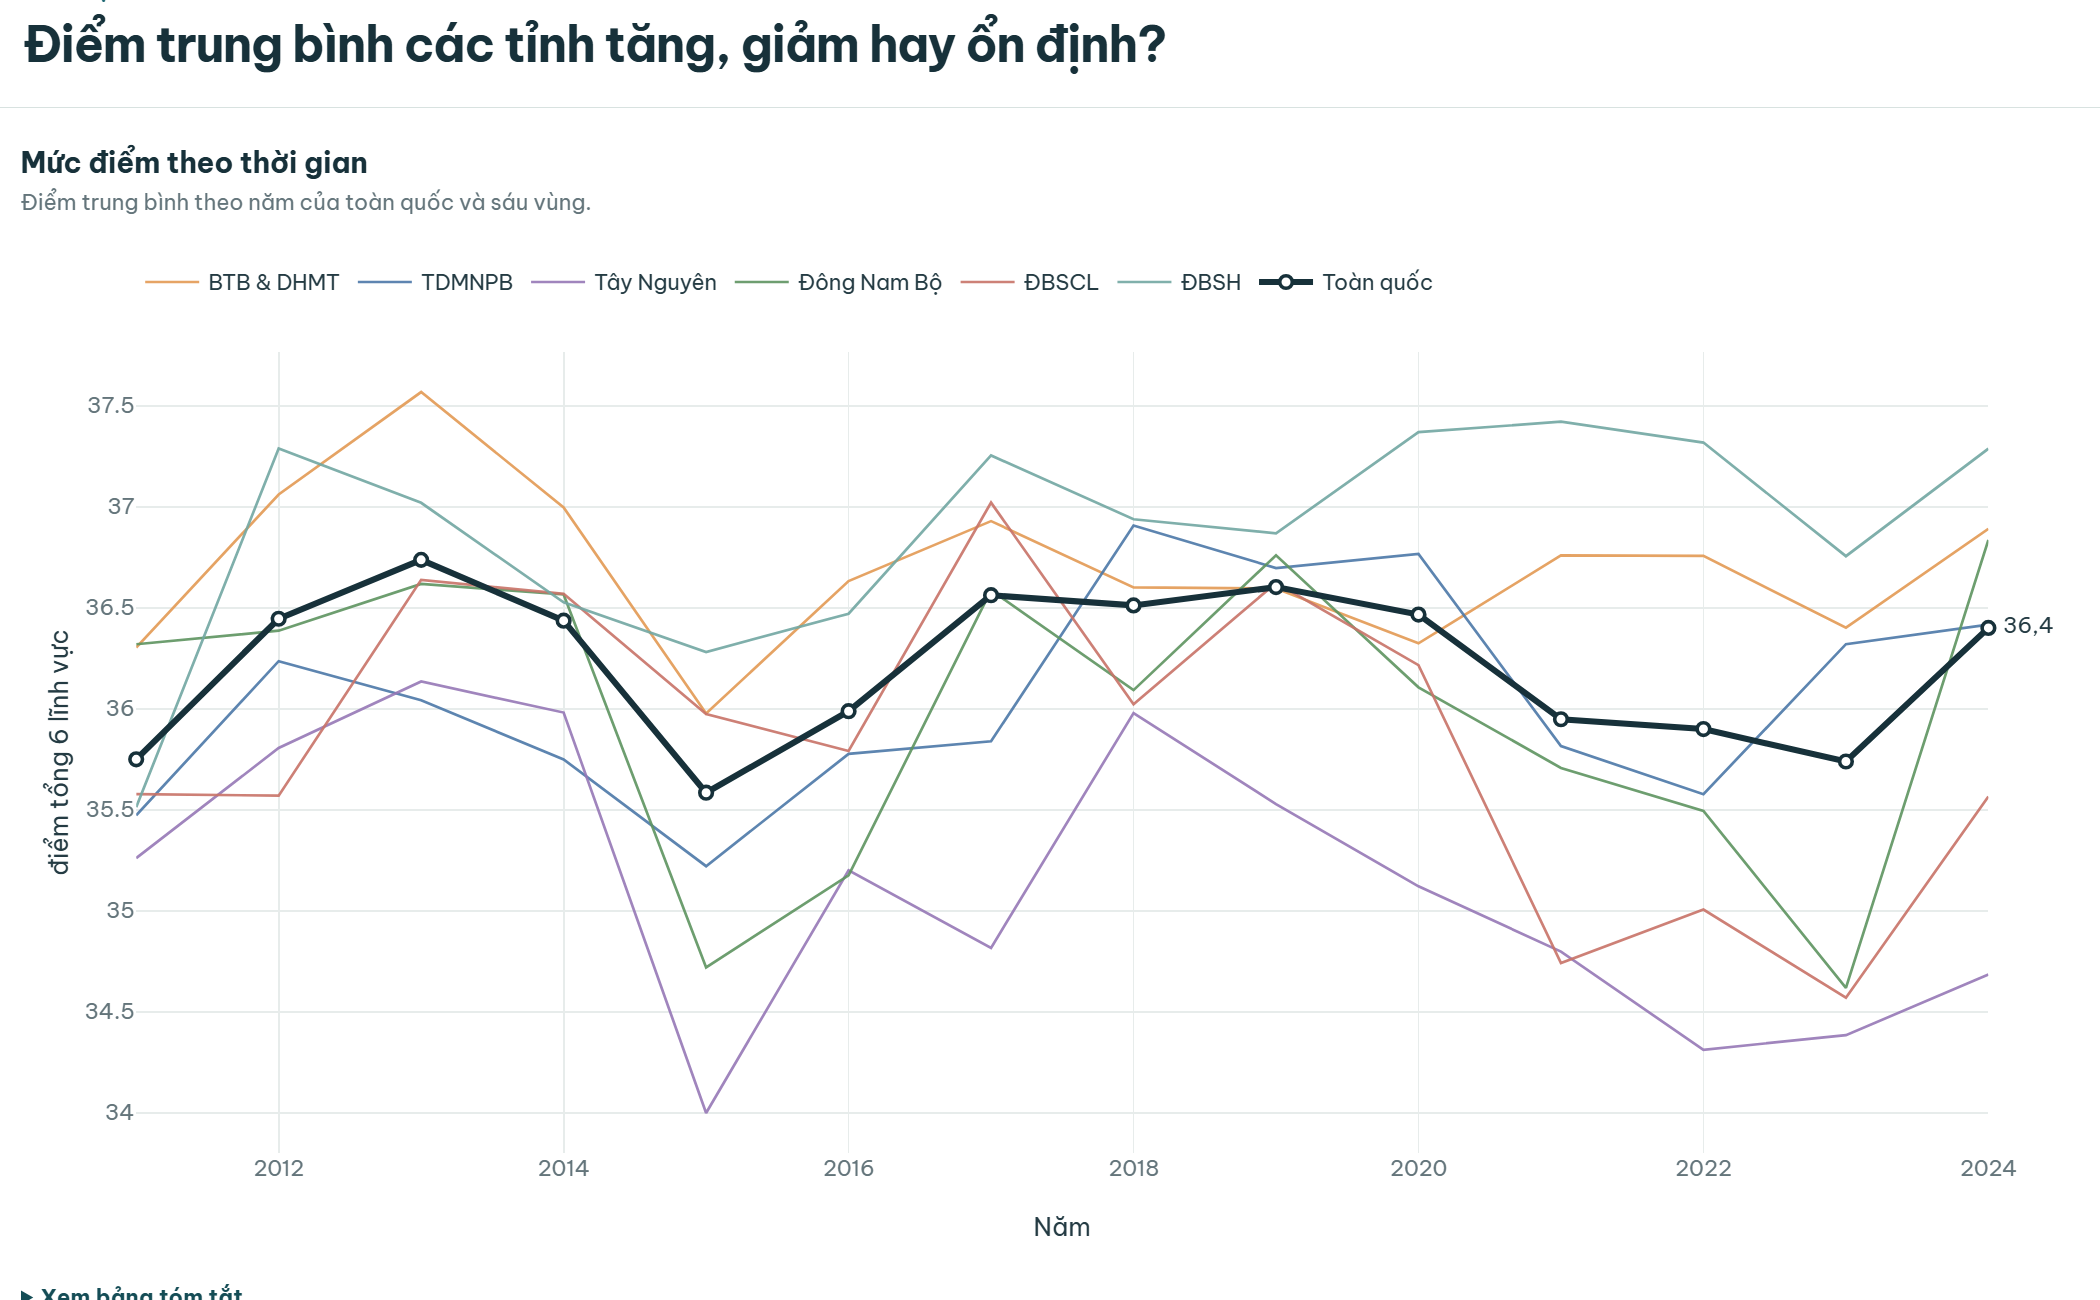
\includegraphics[width=\textwidth,height=0.33\textheight,keepaspectratio]{img/time_series/time_series_total_and_regions_2011_2024.png}
        \caption*{Biểu đồ đường: tổng điểm sáu lĩnh vực của toàn quốc và sáu vùng}
      \end{figure}
      \scriptsize
      \begin{itemize}
        \setlength{\itemsep}{3pt}
        \item[-] Toàn quốc tăng từ \textbf{35,75 điểm} năm 2011 lên \textbf{36,74 điểm} năm 2013.
        \item[-] Giảm còn \textbf{35,58 điểm} năm 2015 và đạt \textbf{36,40 điểm} năm 2024.
      \end{itemize}
    \end{column}
    \begin{column}{0.49\textwidth}
      \begin{figure}
        \centering
        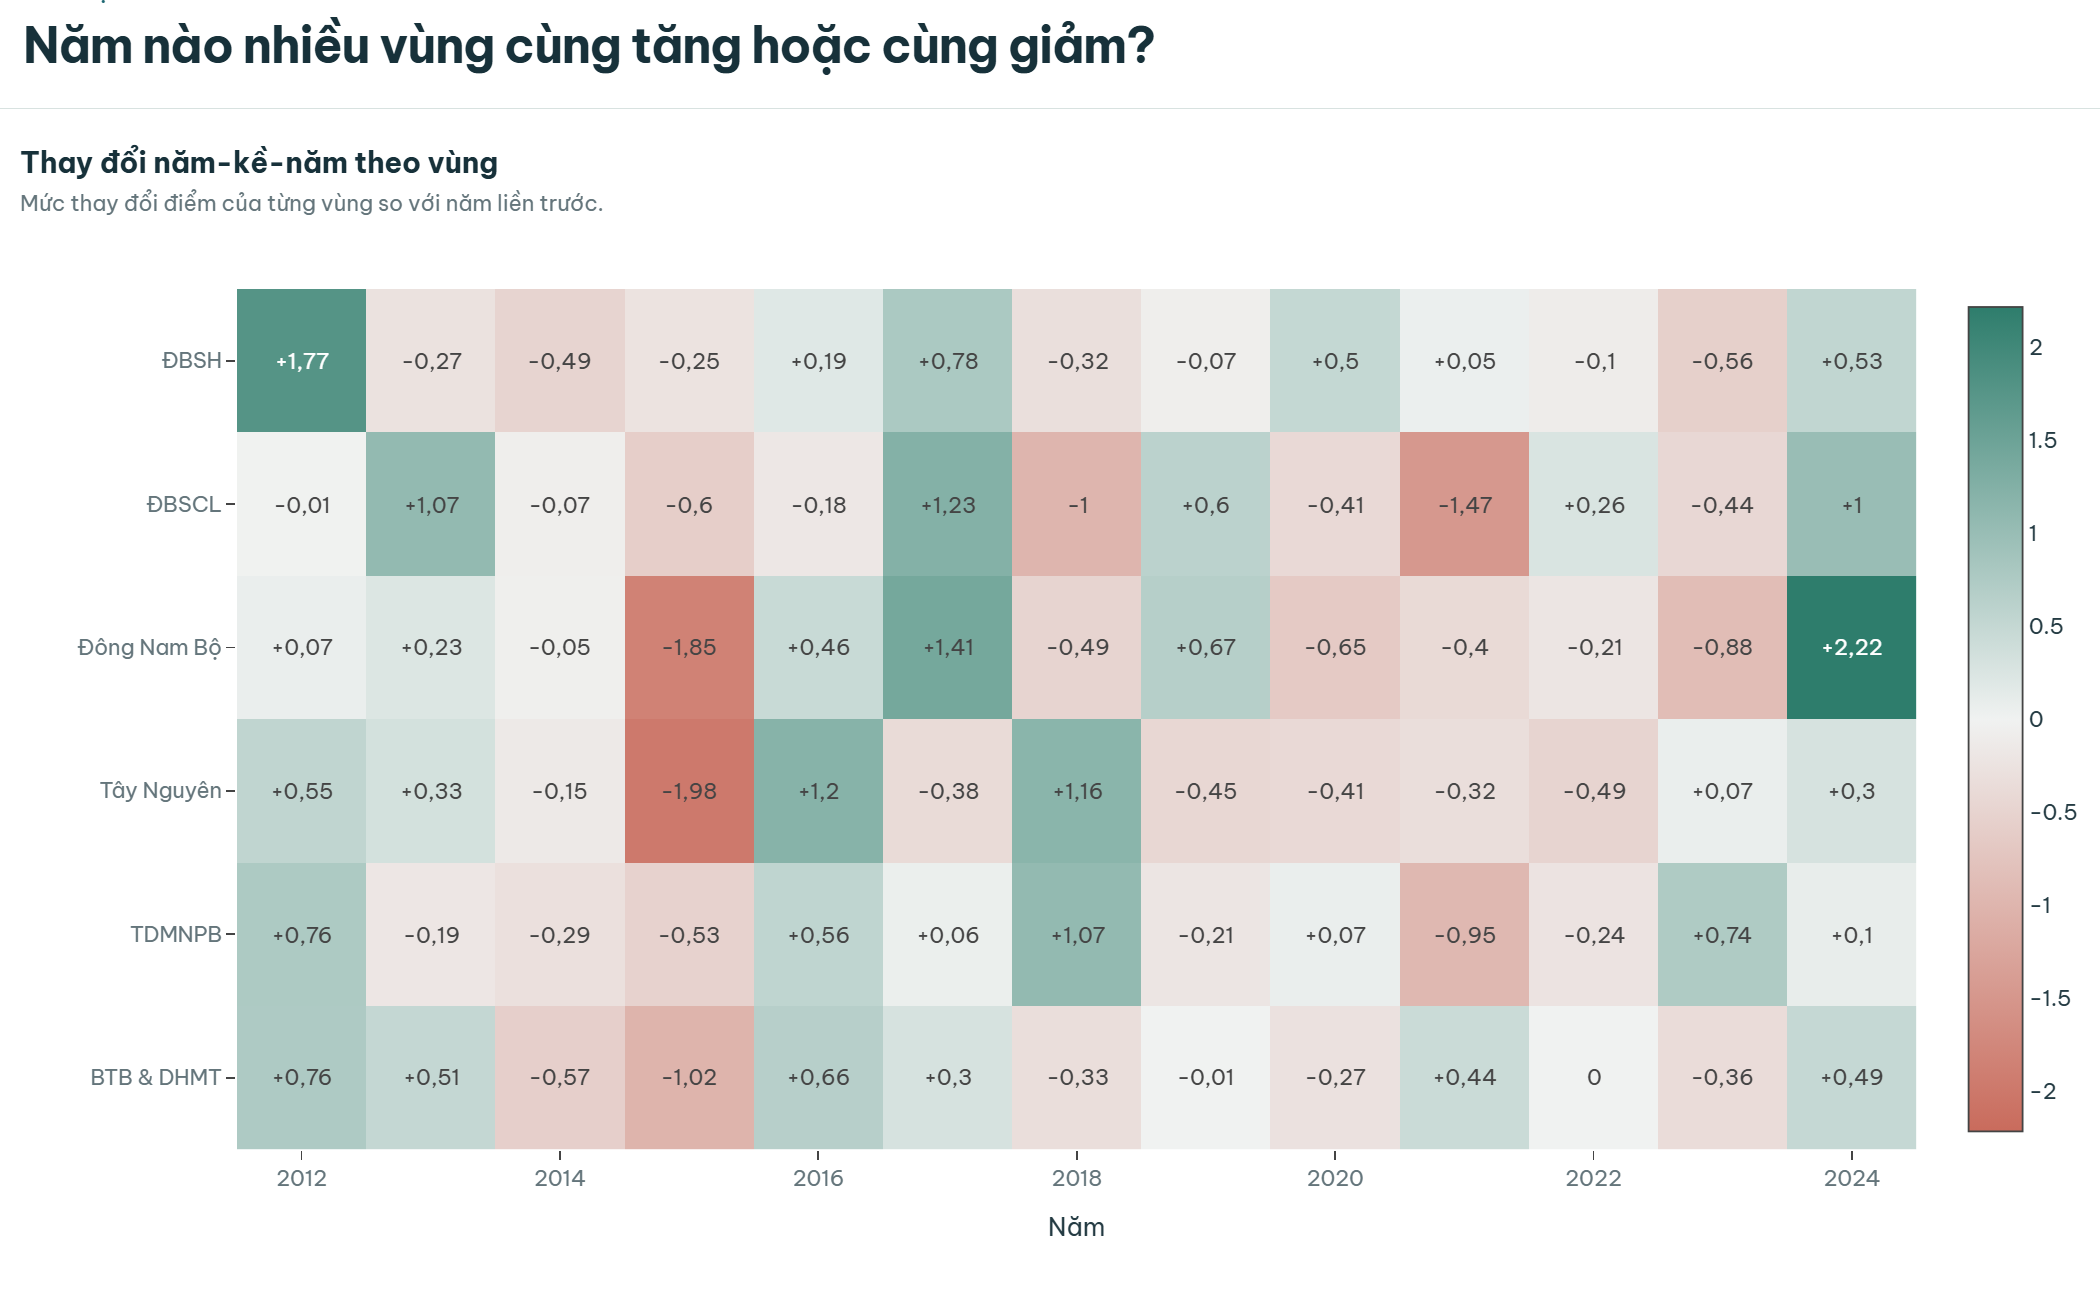
\includegraphics[width=\textwidth,height=0.33\textheight,keepaspectratio]{img/time_series/time_series_regional_yearly_change_2012_2024.png}
        \caption*{Bản đồ nhiệt: mức thay đổi của vùng so với năm trước}
      \end{figure}
      \scriptsize
      \begin{itemize}
        \setlength{\itemsep}{3pt}
        \item[-] Năm \textbf{2015}, cả sáu vùng cùng giảm; Tây Nguyên giảm \textbf{1,98 điểm}.
        \item[-] Năm \textbf{2024}, cả sáu vùng cùng tăng; Đông Nam Bộ tăng \textbf{2,22 điểm}.
      \end{itemize}
    \end{column}
  \end{columns}

\end{frame}

% Slide 11
\begin{frame}[t]{Phân tích Diễn biến theo thời gian}
  \begin{columns}[T,onlytextwidth]
    \begin{column}{0.49\textwidth}
      \begin{figure}
        \centering
        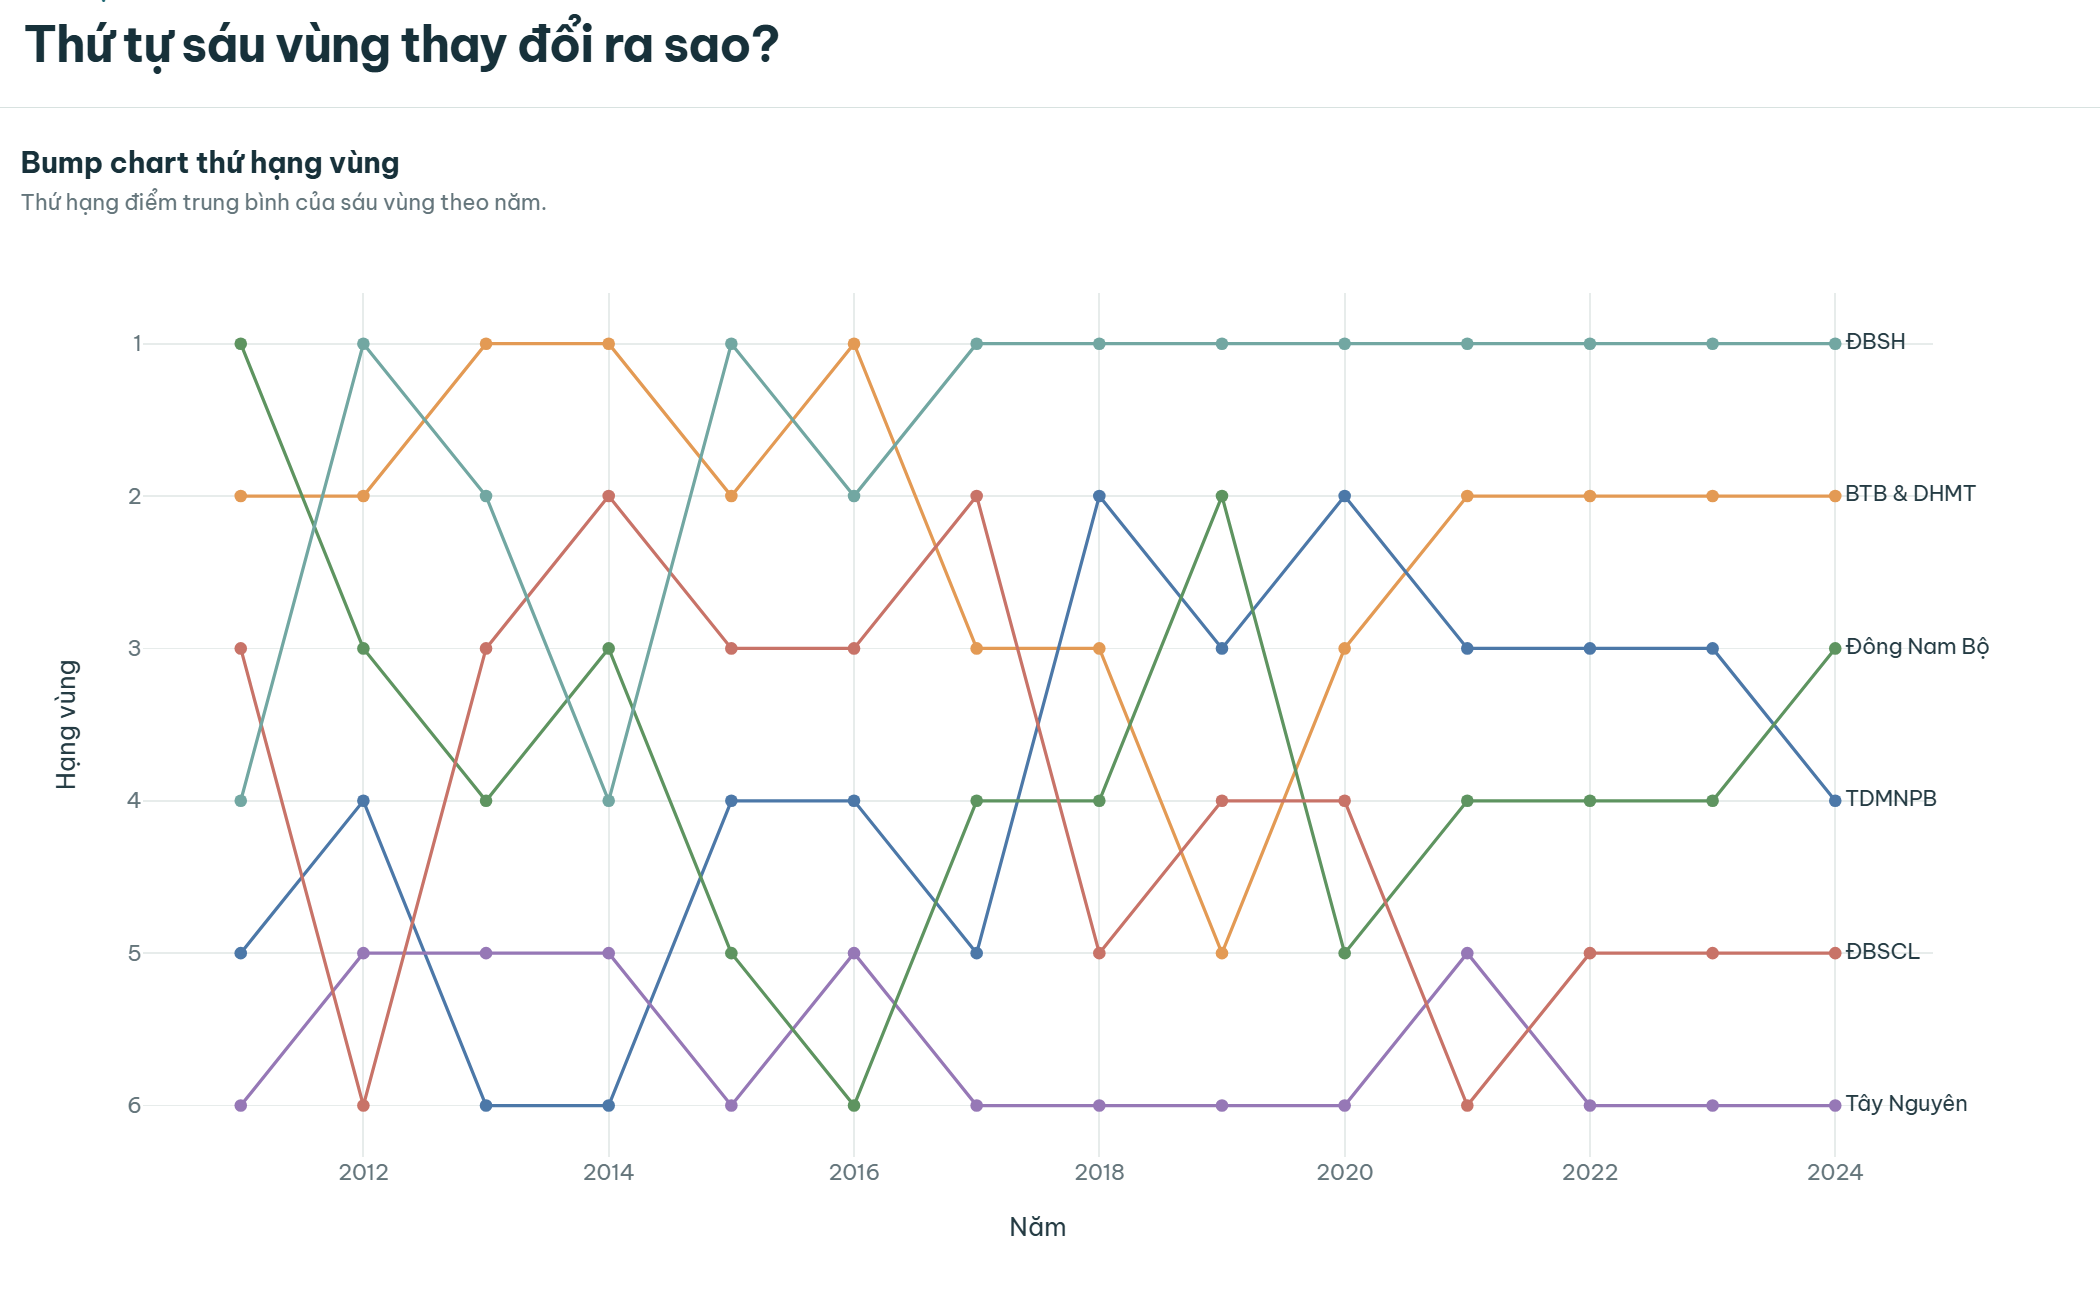
\includegraphics[width=\textwidth,height=0.36\textheight,keepaspectratio]{img/time_series/time_series_regional_rank_2011_2024.png}
        \caption*{Biểu đồ thứ hạng: chuyển dịch giữa sáu vùng}
      \end{figure}
      \scriptsize
      \begin{itemize}
        \setlength{\itemsep}{3pt}
        \item[-] Đồng bằng sông Hồng từ \textbf{hạng 4} lên \textbf{hạng 1} và dẫn đầu từ năm \textbf{2017}.
        \item[-] Tây Nguyên phần lớn nằm ở nhóm cuối.
      \end{itemize}
    \end{column}
    \begin{column}{0.49\textwidth}
      \begin{figure}
        \centering
        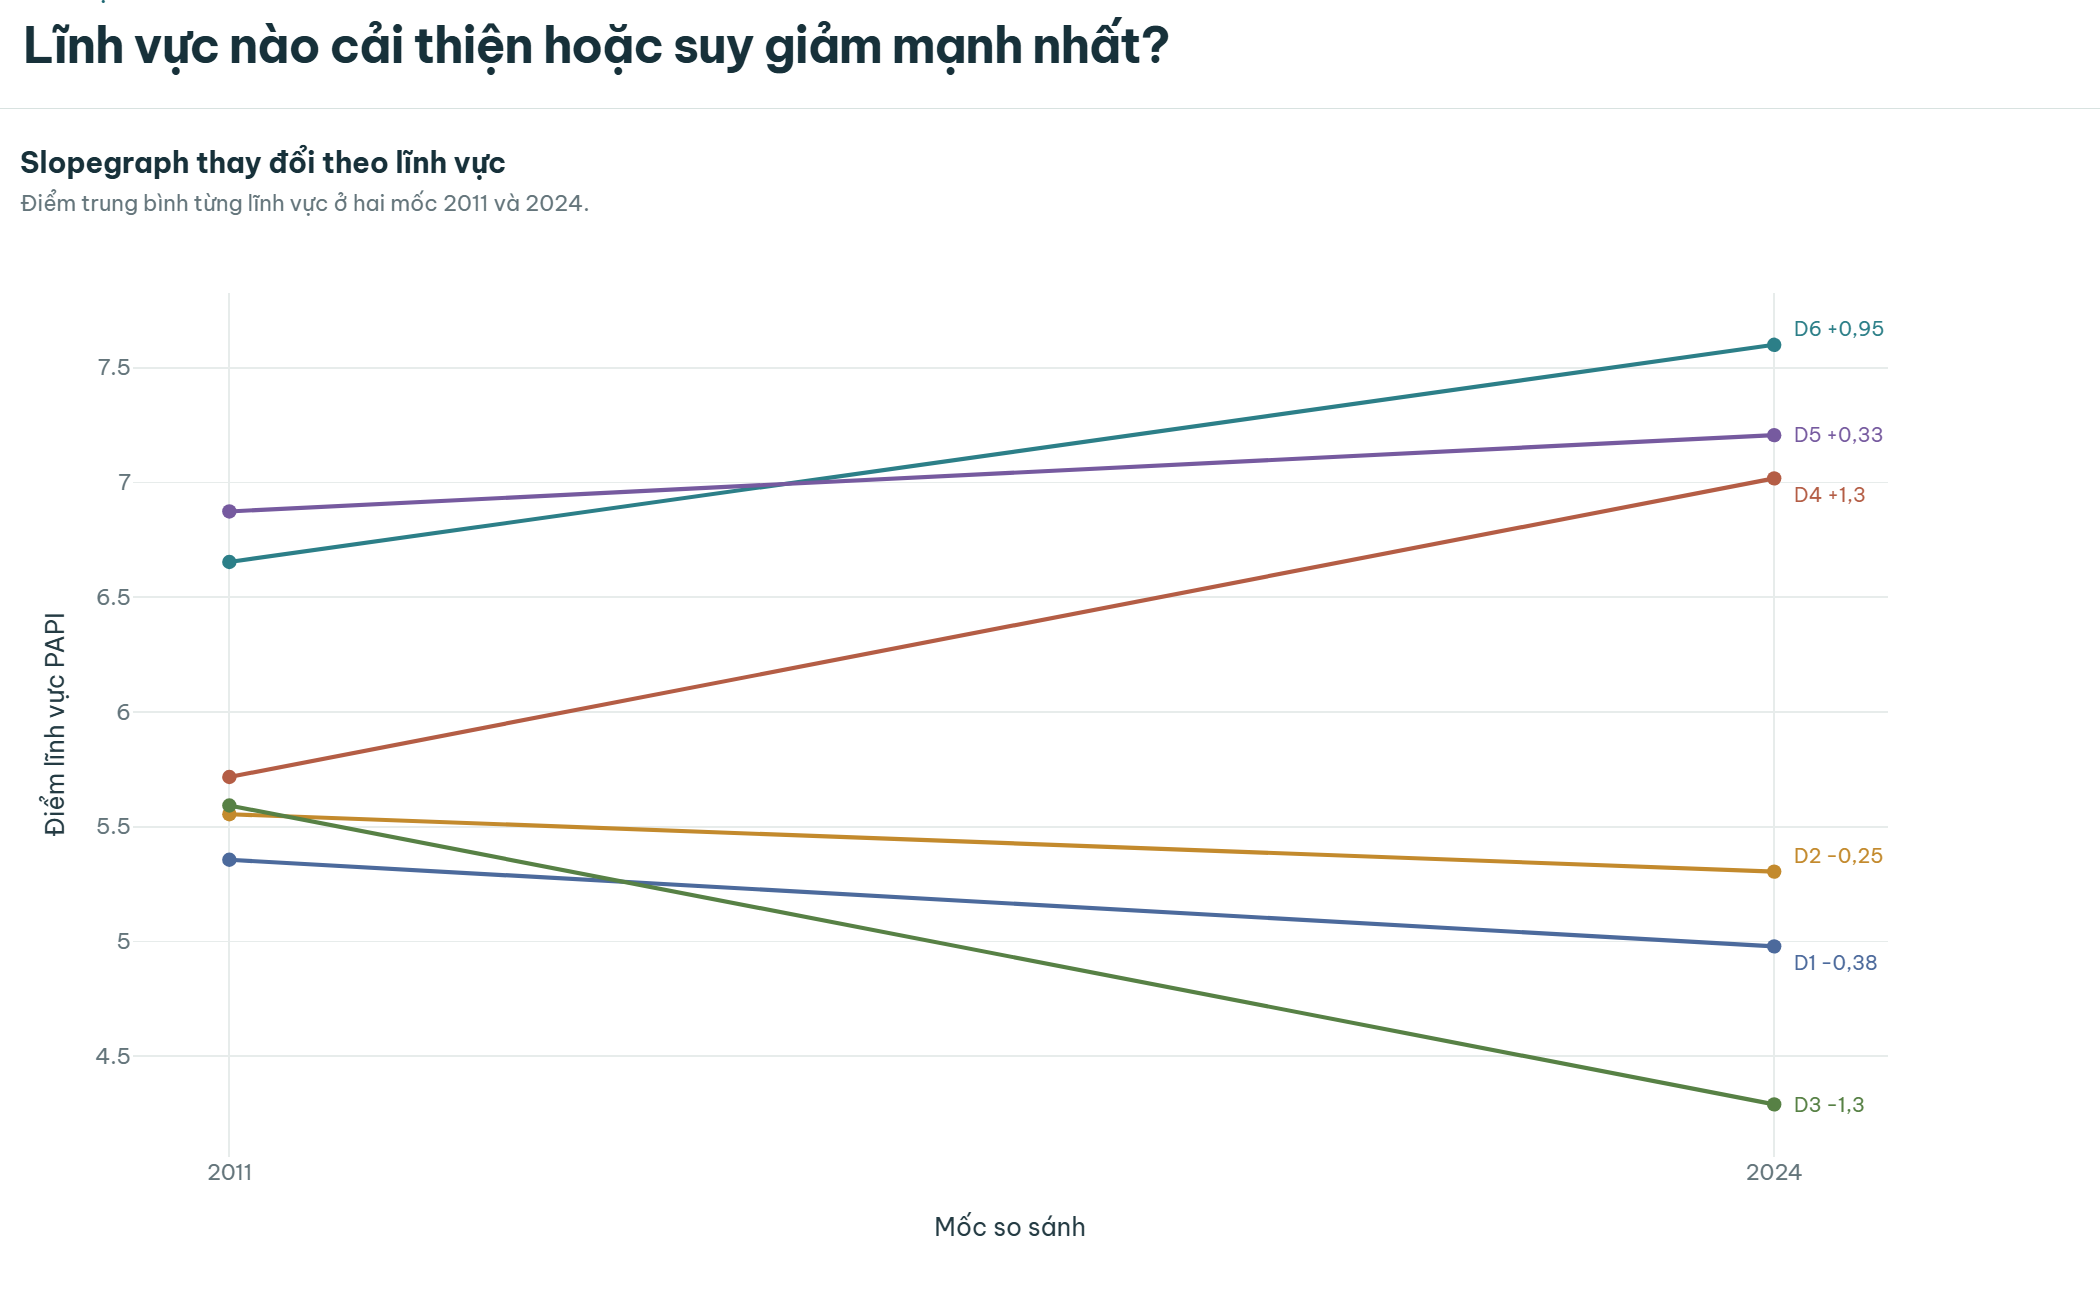
\includegraphics[width=\textwidth,height=0.36\textheight,keepaspectratio]{img/time_series/time_series_dimension_change_2011_2024.png}
        \caption*{Biểu đồ nối hai mốc: thay đổi D1-D6}
      \end{figure}
      \scriptsize
      \begin{itemize}
        \setlength{\itemsep}{3pt}
        \item[-] \textbf{D4} tăng \textbf{1,30 điểm}; \textbf{D6} tăng \textbf{0,95 điểm}.
        \item[-] \textbf{D3} giảm \textbf{1,30 điểm}; D1 và D2 cùng giảm nhẹ.
      \end{itemize}
    \end{column}
  \end{columns}

  \vspace{0.02cm}
  \analysisdirection{%
    phân rã biến động năm 2015 và 2024 theo tỉnh, vùng và lĩnh vực; ưu tiên trách nhiệm giải trình,
    đồng thời duy trì tiến bộ về kiểm soát tham nhũng và dịch vụ công.
  }
\end{frame}
